\documentclass[11pt]{article}
\usepackage{amsfonts,amssymb,amsthm,eucal,amsmath}
\usepackage{graphicx}
\usepackage[T1]{fontenc}
\usepackage{latexsym,url}
\usepackage{array}
\usepackage{subfig}
\usepackage{comment}
\usepackage{color}
\usepackage{tikz}
\usepackage{cprotect}
\usepackage{hyperref}
\usepackage[nameinlink,noabbrev]{cleveref}

\hypersetup{colorlinks=true,linkcolor=blue}
\newcommand{\myspace}{\vspace{.1in}\noindent}
\newcommand{\mymyspace}{\vspace{.1in}}
\usepackage[inner=30mm, outer=30mm, textheight=225mm]{geometry}
\creflabelformat{equation}{#2(#1)#3}
\crefname{equation}{}{}
\Crefname{equation}{}{}

\newtheorem{theorem}{Theorem}[section]
\newtheorem{prop}[theorem]{Proposition}
\newtheorem{corollary}[theorem]{Corollary}
\newtheorem{defn}[theorem]{Definition}
\newtheorem{notn}[theorem]{Notation}
\newtheorem{cond}[theorem]{Condition}
\newtheorem{ex}[theorem]{Example}
\newtheorem{rmk}[theorem]{Remark}
\newcommand{\co}{\negthinspace :}
\newcommand{\N}{\mathbb{N}}
\newcommand{\Z}{\mathbb{Z}}
\newcommand{\R}{\mathbb{R}}
\newcommand{\C}{\mathbb{C}}
\newcommand{\CP}{\mathbb{CP}}
\newcommand{\PSL}{\mathrm{PSL}_2(\mathbb{C})}
\newcommand{\area}{\operatorname{area}}
\newcommand{\diag}{\operatorname{diag}}
\newcommand{\nt}{\negthinspace}
\newcommand{\TODO}{{\color{red} TODO}}

\title{A linear time direct solver for convex tridiagonal quadratic programs with bound constraints}
\author{Geoffrey Irving\thanks{Email: \{irving,keith,martin\}@otherlab.com, Otherlab, San Francisco, CA, United States}
\and Keith Pasko$^*$
\and Martin Wicke$^*$}
\date{Version 1, \today}

\begin{document}
\maketitle

\begin{abstract}
We present a linear time direct solver for symmetric positive definite tridiagonal quadratic programming with bound constraints.  Our algorithm is similar in structure to the
algorithm for linear time shortest paths in triangulated simple polygons by Lee and Preparata.  The algorithm is generalizable to other nonlinear convex programs of similar
structure, though we do not know of any such examples.
\end{abstract}

\section{Background}

Consider a symmetric positive definite tridiagonal quadratic program with bound constraints
\begin{align} \label{qp}
\begin{array}{cc}
\min          \qquad& \frac{1}{2} x^T A x + b^T x \\
\textrm{s.t.} & l \le x \le u
\end{array}
\end{align}
where $x,l,u \in \R^n$ and $A \in \R^{n \times n}$ is symmetric positive definite tridiagonal.  The problem is feasible iff $l \le u$, and can be solved efficiently using an interior point method (see \cite{gondzio2012interior}
for a survey).  Each Newton iteration requires an $O(n)$ tridiagonal direct solve; since interior point methods typically take between $O(1)$ and $O(\log n)$ iterations to converge \cite{colombo2008further}
this results in a quite fast method overall.  However, this peformance is not guaranteed, and any iterative method will require more iterations if greater accuracy is required.

In this paper, we present a linear time direct solver specialized for \cref{qp}.  We discovered this algorithm by accident: we intended to derive an linear time algorithm
for shortest paths (geodesics) in triangle strips immersed in three dimensions, but mistakenly wrote down a sum of squared lengths instead of the correct sum of unsquared lengths.  We then arrived at a linear time algorithm
using geometric intuition before realizing that our motivating problem was not a quadratic program after all.  In fact, essentially the same algorithm works in both cases, although an extra data structure is required
for quadratic programming.  The shortest path case is due to Lee and Preparata \cite{lee1984euclidean}, but to our knowledge its application to quadratic programming is unpublished.

We review the geometric case first.  Consider a sequence of segments $p_i q_i$ with $p_i, q_i \in \R^2$ for $i = 0, \ldots, n$, forming a quadrilateral strip.  Place an interpolated point
$r_i = (1-t_i) p_i + t_i q_i$ on each segment, where $0 \le t_i \le 1$.  Assume that the first and last points are fixed, so that $p_0 = q_0$ and $p_n = q_n$, and that each quadrilateral is convex.
We seek to minimize the total length
\begin{align*}
L &= \sum_{i=0}^{n-1} \left\| r_i - r_{i+1} \right\|.
\end{align*}
The algorithm proceeds from $k = 0$ to $k = n-1$, where stage $k$ minimizes the length up to $r_k$ for the two extreme values $r_k = p_k, q_k$.  Since segments do not intersect, the optimal value
of $t_i$ for $i < k$ is a monotonic function of $x_k$, so the optimal path for any intermediate value $0 < t_k < 1$ lies between the optimal paths for $t_k = 0,1$.  Thus, our intermediate state has the form shown in
\cref{kite}: the two paths stay together for a certain distance, then curve apart in opposite directions.  Moving from $k$ to $k+1$ consists of adding new edges to each path, then eroding until
we restore convexity.  To determine whether to remove a vertex at index $j$ between $i$ and $k$, we compute a shortest path between $r_i$ and $r_k$ and compare it to the bounds on $r_j$, which takes $O(1)$ time.
For full details, see \cite{lee1984euclidean}.

\begin{figure}
\begin{center}
\begin{tikzpicture}[thick,line join=round,line cap=round,scale=.7]
  \draw (-6,.1) node[left]{$r_0$} -- (-4.5,1) -- (-3,-.2)  -- (-1.5,.7) -- (0,0) node[above]{$r_j$}; % shared
  \draw (0,0) -- (1.8,.6) -- (3.3,1.6) -- (4.2,3.5) node[right]{$p_k$};      % upper
  \draw (0,0) -- (1.5,-.4) -- (3,-1.6) -- (4.2,-3.5) node[right]{$q_k$};     % lower
\end{tikzpicture}
\end{center}
\caption{Intermediate state of the linear time algorithm for shortest paths in quadrilateral strips.  The lower and upper parts stay together from $r_0$ to $r_j$, and then diverge in different directions
following the active constraints $p_i$ and $q_i$. \label{kite}}
\end{figure}

\section{Tridiagonal quadratic programs}

On to the quadratic program \cref{qp}.  We first use the Cholesky decomposition $A = L L^T$ to convert the quadratic energy into a sum of energies of adjacent variables:
\begin{align*}
E &= \frac{1}{2} x^T A x + b^T x  \\
  &= \frac{1}{2} x^T L L^T x + b^T x \\
  &= \frac{1}{2} \left\|L^T x + L^{-1}b \right\|^2 - \frac{1}{2} b^T L^{-T} L^{-1} b \\
  &= \sum_{i=0}^{n-1} E_{i,i+1}(x_i,x_{i+1}) + \textrm{const}
\end{align*}
using
\begin{align} \label{quadratic}
E_{i,i+1}(x_i,x_{i+1}) = \frac{1}{2} (L_{i,i} x_i + L_{i+1,i} x_{i+1} + c_i)^2
\end{align}
where we have introduced sentinels $x_{n+1} = L_{n+1,n} = 0$ for notational simplicity.  We sweep through adjusting the signs of each $x_i$ so that $L_{i+1,i} \le 0$; since $L_{i,i} > 0$, this
ensures that the local optimal value of $x_i$ is a weakly increasing function of $x_{i-1}$ and $x_{i+1}$.

For any $0 \le i < k \le n$, define a function $E_{ik}$ by partially minimizing over all variables strictly between $x_i$ and $x_k$:
$$E_{ik}(x_i,x_k) = \min_{x_{i+1}, \ldots, x_{k-1}} \sum_{j = i}^{k-1} E_{j,j+1}(x_j,x_{j+1}).$$
This minimization produces a linear system for the intermediate $x_j$.  Since substituting a linear function into a quadratic gives a quadratic, each $E_{ik}$ is of the form \cref{quadratic} up to a constant,
and we can combine $E_{ij}$ and $E_{jk}$ into $E_{ik}$ in $O(1)$ time.  $E_{ik}$ encodes the set of optimal paths from $x_i$ to $x_k$ when bound constraints are ignored.

\begin{figure}
\begin{center}
  \tikzset{kite/.style = {thick,line join=round,line cap=round,scale=.5}}
  \begin{tikzpicture}[kite]
    \draw (-6,.1) -- (-4.5,1) -- (-3,-.2)  -- (-1.5,.7) -- (0,0) node[above]{$x_{j_0}$} node[below]{$x_{i_0}$};
    \draw (0,0) -- (2.7,.9) -- (4.2,3.5) node[right]{$u_{k-1}$};
    \draw (0,0) -- (1.5,-.4) -- (3,-1.6) -- (4.2,-3.5) node[right]{$l_{k-1}$};
    \draw (-5.5,-2) node[right]{(1) Start};
  \end{tikzpicture}
  % Erode upper right
  \begin{tikzpicture}[kite]
    \draw (-6,.1) -- (-4.5,1) -- (-3,-.2)  -- (-1.5,.7) -- (0,0) node[name=base]{};
    \draw (0,0) -- (2.7,.9) -- (4.2,3.5) -- (5,-2.2) node[name=up,right]{$u_k$};
    \draw (0,0) -- (1.5,-.4) -- (3,-1.6) -- (4.2,-3.5) -- (5,-3.8) node[name=down,right]{$l_k$};
    \draw[red] (2.7,.9) -- (5,-2.2);
    \filldraw[red] (4.2,3.5) circle (5pt);
    \draw (-5.5,-2) node[right]{(2) Erode upper right};
  \end{tikzpicture}
  \begin{tikzpicture}[kite]
    \draw (-6,.1) -- (-4.5,1) -- (-3,-.2)  -- (-1.5,.7) -- (0,0) node[name=base]{};
    \draw (0,0) -- (2.7,.9) -- (5,-2.2) node[name=up,right]{$u_k$};
    \draw (0,0) -- (1.5,-.4) -- (3,-1.6) -- (4.2,-3.5) -- (5,-3.8) node[name=down,right]{$l_k$};
    \draw[red] (0,0) -- (5,-2.2);
    \filldraw[red] (2.7,.9) circle (5pt);
    \draw (-5.5,-2) node[right]{(3) Erode upper right};
  \end{tikzpicture}
  % Erode lower left
  \begin{tikzpicture}[kite]
    \draw (-6,.1) -- (-4.5,1) -- (-3,-.2)  -- (-1.5,.7) -- (0,0) node[name=base]{};
    \draw (0,0) -- (1.5,-.4) -- (3,-1.6) -- (4.2,-3.5) -- (5,-3.8) node[name=down,right]{$l_k$};
    \draw[red] (0,0) -- (5,-2.2) node[name=up,right,black]{$u_k$};
    \filldraw[red] (1.5,-.4) circle (5pt);
    \draw (-5.5,-2) node[right]{(4) Erode lower left};
  \end{tikzpicture}
  \begin{tikzpicture}[kite]
    \draw (-6,.1) -- (-4.5,1) -- (-3,-.2)  -- (-1.5,.7) -- (0,0) node[name=base]{};
    \draw (0,0) -- (1.5,-.4) -- (3,-1.6) -- (4.2,-3.5) -- (5,-3.8) node[name=down,right]{$l_k$};
    \draw[blue] (1.5,-.4) -- (5,-2.2) node[name=up,right,black]{$u_k$};
    \filldraw[blue] (3,-1.6) circle (5pt);
    \draw (-5.5,-2) node[right]{(5) Lower left done};
  \end{tikzpicture}
  % Erode lower right
  \begin{tikzpicture}[kite]
    \draw (-6,.1) -- (-4.5,1) -- (-3,-.2)  -- (-1.5,.7) -- (0,0) node[name=base]{};
    \draw (1.5,-.4) -- (5,-2.2) node[name=up,right]{$u_k$};
    \draw (0,0) -- (1.5,-.4) -- (3,-1.6) -- (4.2,-3.5) -- (5,-3.8) node[name=down,right]{$l_k$};
    \draw[red] (3,-1.6) -- (5,-3.8);
    \filldraw[red] (4.2,-3.5) circle (5pt);
    \draw (-5.5,-2) node[right]{(6) Erode lower right};
  \end{tikzpicture}
  \begin{tikzpicture}[kite]
    \draw (-6,.1) -- (-4.5,1) -- (-3,-.2)  -- (-1.5,.7) -- (0,0) node[name=base]{};
    \draw (1.5,-.4) -- (5,-2.2) node[name=up,right]{$u_k$};
    \draw (0,0) -- (1.5,-.4) -- (3,-1.6) -- (5,-3.8) node[name=down,right]{$l_k$};
    \draw[blue] (1.5,-.4) -- (5,-3.8);
    \filldraw[blue] (3,-1.6) circle (5pt);
    \draw (-5.5,-2) node[right]{(7) Lower right done};
  \end{tikzpicture}
  \begin{tikzpicture}[kite]
    \draw (-6,.1) -- (-4.5,1) -- (-3,-.2)  -- (-1.5,.7) -- (0,0) node[name=base]{};
    \draw (1.5,-.4) -- (5,-2.2) node[name=up,right]{$u_k$};
    \draw (0,0) -- (1.5,-.4) -- (3,-1.6) -- (5,-3.8) node[name=down,right]{$l_k$};
    \draw (-5.5,-2) node[right]{(8) Finished};
  \end{tikzpicture}
\end{center}
\caption{A single step of the algorithm, drawn as if we were computing shortest paths.
(1) We start from two paths ending at the $(k-1)$th lower and upper constraints.
(2-3) The two paths are extended by adding $l_k$ and $u_k$ on the right, and the upper path is eroded from the right as far as possible.
(4-5) Since the upper path erodes to a single line, we erode the lower path from the left using the upper $u_k$ constraint.
(6-8) The lower path is eroded from the right in the same manner, arriving at the final $k$th state.
\label{erode}}
\end{figure}

As in the geometric case, our algorithm proceeds from $k = 0$ to $k = n-1$, maintaining two minimizers of the partial energy up to $x_k = l_k$ and $x_k = u_k$.  We represent the two partial minimizers in terms of
their active constraints.  The $x_k = l_k$ and $x_k = u_k$ paths will agree up to a certain $x_j$, then deviate
in opposite directions with the $x_k = l_k$ path touching only $l_i$ constraints and the $x_k = u_k$ path touching only $u_i$ constraints.  To advance from $k$ to $k+1$, we extend the two partial solutions by adding
$l_{k+1}$ and $u_{k+1}$ constraints, respectively, then remove constraints that violate local optimality starting from $l_k$ and $u_k$ until optimality is restored.  If we erode the entire separate
portion of one of our two paths, we continue eroding the beginning of the other separate path, extending the common section of the paths.  This process is illustrated in \cref{erode}.
A constraint is considered for removal only when a neighbor is added or removed, and a constraint is added (resp.\ removed) at most once.  Thus, assuming we know the appropriate $E_{ij}$ when we need them, each step
is amortized constant time, and the overall complexity is $O(n)$.

Which $E_{ij}$ do we need?  Let the lower and upper paths have indices $(i_0, i_1, \ldots, i_a)$ and $(j_0, j_1, \ldots, j_b)$, respectively, where $i_0 = j_0$ is the last shared vertex of the paths
and $i_a = j_b = k$ is the index just added.  When eroding the lower path from the left, we need energy terms $E_{i_{a-2}i_{a-1}}$ and $E_{i_{a-1}i_{a}}$, which are available if we maintain
energy terms between all adjacent indices $E_{i_0i_1}, E_{i_1i_2}, \ldots$ along the path.  When a new index is appended on the left we add a new energy term along with it, and if index $i_{a-1}$ is
eliminated we reduce $E_{i_{a-2}i_{a-1}}$ and $E_{i_{a-1}i_{a}}$ into $E_{i_{a-2},i_a}$ in $O(1)$ time.

If we erode the entire lower path down to $(i_0,i_a)$ and start eroding the upper path $(j_0, j_1, \ldots, j_b)$, our decision depends on the energy terms $E_{j_0j_1}$ and $E_{j_1i_a} = E_{j_1j_b}$.
Thus, in addition to consecutive energy terms we need the term $E_{j_1j_b}$ crossing the entire disjoint portion of the path.  This amounts to maintaining the product of a queue of semigroup elements,
and we use a modified version of the ``two stack'' solution of sevenkplus\footnote{CS Theory Stack Exchange, \url{http://cstheory.stackexchange.com/questions/18655}}.  Specifically, we pick a pivot
index $j_1 \le p \le j_b$, store $E_{j p}$ for $j < p$, and store $E_{p j_b}$.  $E_{j_1 j_b}$ is then available by combining $E_{j_1 p}$ with $E_{p j_b}$.  When a new element is appended to the left
we update $E_{p j_b}$.  If index $j_1$ is eliminated nothing need be done unless $p < j_2$, in which case we reset the pivot to $p = j_b$ and recompute all $E_{j p}$ for $j < p$ in reverse order.
This cost is amortized $O(1)$ time by charging the computation of $E_{j p}$ to the append operation which added $j$.  Note that the pivot index is not necessarily part of the path.

This ``semigroup queue'' data structure is unnecessary for shortest paths in polygons because any $E_{ij}$ is available in $O(1)$ time using the coordinates of the input points.  However,
it appears to be impossible to make all the $E_{ij}$ stably available up front for quadratic programming.\footnote{For failed attempts, see \url{http://scicomp.stackexchange.com/questions/8090}.}
This is because the semigroup is not a group: we cannot stably compute $E_{12}$ from $E_{13}$ and $E_{23}$, because the latter
carry no information about $E_{12}$ if $x_2$ and $x_3$ are uncoupled in the linear system.
Fortunately, the semigroup queue allows us to keep track of exactly those energy terms that we need while preserving stability.

\section{Other nonlinear programs}

\begin{figure}[t]
\begin{center}
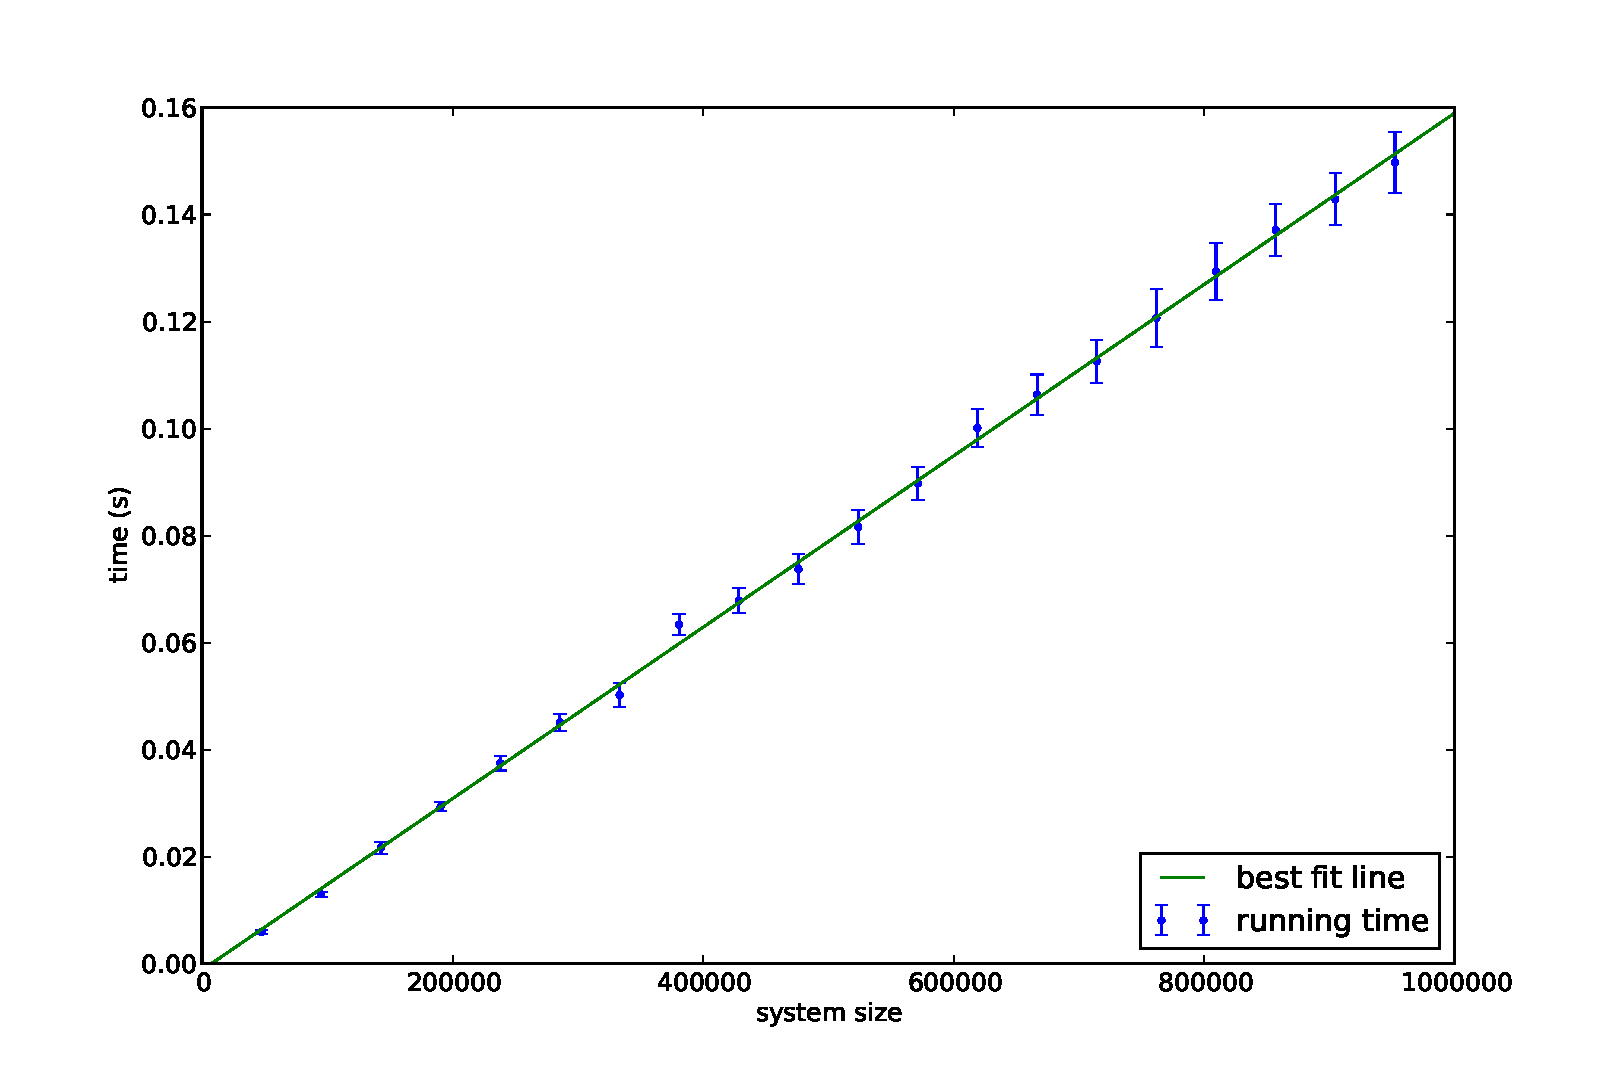
\includegraphics[width=.7\columnwidth]{benchmark.pdf}
\end{center}
\vspace{-.2in}
\cprotect\caption{Benchmark timings for the prototype implementation on a 2.7 GHz Intel Core i7 MacBook Pro.  To reproduce this figure, run \verb+./benchmark --known 1+ in the source repository
(leave out \verb+--known 1+ to regenerate timings).}
\label{benchmark}
\end{figure}

Expressed in terms of energy functions, our algorithm solves the optimization problem
\begin{align*}
\begin{array}{cc}
\min          \qquad& \sum E_{i,i+1}(x_i,x_{i+1}) \\
\textrm{s.t.} & l \le x \le u
\end{array}
\end{align*}
Define $E_{ij}$ as above.  The algorithm works in $O(n)$ time if the following properties hold:
\begin{enumerate}
\item For any $i < j < k$, we can combine $E_{ij}$ and $E_{jk}$ into $E_{ik}$ in $O(1)$ time.
\item Given $E_{ij}$, $E_{jk}$, $x_i$, and $x_k$, we can compute the optimum value of $x_j$ in $O(1)$ time.
\item For $i < j < k$, $x_j$ is a monotonic function of $x_i$ and $x_k$.
\end{enumerate}
Unfortunately, the first property is quite fragile, and we do not know of any useful examples beyond shortest paths in polygons and tridiagonal quadratic programming.  For example, if the index of
refraction is allowed to vary across quadrilaterals in a quad strip for a shortest path problem, we can no longer combine $E_{ij}$ with $E_{jk}$ in $O(1)$ time, and the algorithm fails.

\section{Implementation}

A prototype implementation of the algorithm is available under a BSD-style license at \url{https://github.com/otherlab/tridiagonal}, along with the latex source of the paper.
The core algorithm is implemented in \verb+module.cpp:tridiagonal_qp()+.  As shown in \cref{benchmark}, the implementation is linear time in practice.  Git commit 
\verb+282e5cd3fb86d+ was used for the benchmark.

\bibliography{references}
\bibliographystyle{acm}

\end{document}
